\chapter{Planificación e Seguimento}

A elaboración deste proxecto levouse a cabo durante tres períodos de tempo diferenciados e separados no tempo:

\begin{itemize}
  \item O verán do ano 2013 como parte do programa GSoC.
  \item O primeiro cuatrimestre do curso 2013/2014.
  \item O verán do ano 2014 novamente como parte do GSoC.
\end{itemize}

Neste capítulo trataremos a planificación do proxecto e como se levou a cabo neses catro períodos de tempo.

\section{Google Summer of Code 2013}
A duración do período do traballo programando do Google Summer of Code son aproximadamente 4 meses, un total de 15 semanas. Durante a edición de 2013 planificase que se traballa 13 semanas. As dúas semanas restantes corresponden a asistencia a GUADEC e ao comezo do ano lectivo universitario 2013/2014. Contase traballar aproximadamente 5 horas diarias o que dá un total de 325 horas.

O programa GSoC pide os participantes reportes periódicos en forma de artigos en blogues así que estas serán as nosas iteracións a través das cales iremos recibindo feedback por parte dos futuros usuarios do aplicativo. En función deste feedback iremos modificando o programa. Neste caso empregarase un blogue persoal creado con anterioridade e de nome \href{http://aquelando.info}{Aquelando.info}. As publicacións deste blogue así como as de moitos desenvolvedores do proxecto GNOME están ligadas con Planet GNOME, que é un agregador de blogues, polo que a súa difusión é moi alta. A periodicidade das publicacións e polo tanto das iteracións variará dunha a outra pero é de entre dúas e tres semanas.

Durante este GSoC fixéronse 5 iteracións que explicamos a continuación.

\subsection{Primeira Iteración: Análise, deseño xenérico e inicio da implementación}

A primeira iteración iníciase o 13 de Xuño e rematará o 30 de Xuño. O obxectivo desta primeira iteración é facer unha análise das necesidades dos tradutores e realizar un deseño xenérico da estrutura do programa.

\paragraph{Análise e deseño}
Para a análise de requisitos, instalaranse e estudaranse as características de algúns dos programas do mercado. Ademais contactaremos con diversos equipos de tradución a través das súas listas de correo. Unha vez que se obteña certo feedback por parte dos equipos comezarase a realizar un deseño xenérico da estrutura do programa.

\paragraph{Implementación da clase abstracta ficheiro}
Empezarase a implementar parte do núcleo do sistema en concreto unha clase abstracta ficheiro e unha clase \emph{DemoFile} que servirá como \emph{mock} para poder implementar a interface. Para a implementación desta clase terase en conta o concerto de extensibilidade xa que este programa aínda que se centrará na edición de ficheiros PO por ser estes os ``oficiais'' de GNOME tamén queremos que este programa sexa útil para a comunidade de tradutores en xeral.

\subsubsection{Reporte e feedback}
Escribíronse un total de 3 reportes. Un\footnote{\href{http://aquelando.info/startinggsocprojec/}{Starting the GSoC Project!!}} facendo referencia as peticións obtidas por parte dos equipos de tradución e dous\footnote{\href{http://aquelando.info/valacat-some-design-aspects/}{ValaCAT. Some design aspects}}\footnote{\href{http://aquelando.info/valacat-some-design-aspects-part-2/}{ValaCAT. Some design aspects (Part 2)}} con algúns detalles que se tiveron en conta durante o deseño do programa. Houbo bastantes comentarios no blogue e entre outras cousas os usuarios destacaron:

\begin{itemize}
  \item A importancia de non usar o patrón Singleton.
  \item Non facer os widgets dependentes da aplicación para que istos poidan ser reutilizados en outras aplicacións como Anjuta.
  \item Usar gettext-po para implementar os ficheiros po.
  \item Empregar unha interface máis semellante a anterior de GTranslator.
  \item Eliminar a columna de ID pois non se considera útil.
  \item Autoexpandir o tamaño dos campos cando as cadeas sexan grandes.
\end{itemize}

Con respecto a estas ideas modificouse a interface que se ía facer para buscar un deseño moi parecido ao de GTranslator empregando ingluso a mesma biblioteca GNOME Docking Library que permite modificar os bloques da interface. Ademais eliminouse por completo o ID da cadea da interface. En canto a biblioteca gettext-po xa tiñamos en mente empregala.

\subsubsection{Tarefas e seguimento}

A descomposición de tarefas desta iteración é a segunte:

\begin{enumerate}[label=\bfseries WBS 1.\arabic*]
  \item Análise de Requisitos
    \begin{enumerate}[label=\bfseries WBS 1.1.\arabic*]
      \item Estudio de ferramentas existentes.
      \item Enviar correos a diferentes equipos de tradutores.
      \item Analizar respostas dos equipos.
    \end{enumerate}
  \item Deseño xenérico do aplicativo.
  \item Deseño e implementación do ficheiros xenérico.
  \item Escribir primeiros reportes.
\end{enumerate}

Ao igual que sucederá en todo este proxecto a planificación destas tarefas é lineal pois so dispoñemos dun recurso. Na Figura~\ref{fig:gantt:gsoc1-1} pódese ver o diagrama de Gantt que correponde a esta iteración.

\begin{figure}[h!]
\centerline{
\begin{ganttchart}[
    %hgrid,
    %inline,
    vgrid={dotted,dotted, dotted, dashed, dashed, dotted, dotted},
    x unit=5mm,
    y unit title=5mm,
    y unit chart=6mm,
    canvas/.style={draw=none},
    time slot format=isodate,
    title/.style={fill=gray, draw=none},
    title label font= \color{white}\scriptsize,
    title left shift=.1,
    title right shift=-.1,
    title top shift=.05,
    title height=.5,
    bar label font=\scriptsize,
    milestone label font=\scriptsize,
    group label font=\scriptsize\bfseries,
    %milestone inline label node/.append style={bottom=5mm},
    %group inline label node/.append style={right=0mm},
    %bar inline label node/.append style={right=0mm}
  ]{2013-06-11}{2013-6-29}
  \gantttitlecalendar{month=name,day} \\
  \ganttgroup{Análise de Requisitos}{2013-06-12}{2013-06-19} \\
  \ganttbar{Enviar correos a equipos de tradutores}{2013-06-12}{2013-06-13} \\
  \ganttlinkedbar{Analizar respostas dos equipos}{2013-06-18}{2013-06-19} \\
  \ganttbar{Estudo de ferramentas existentes}{2013-06-16}{2013-06-17} \\
  \ganttlinkedbar{Deseño xenérico do aplicativo}{2013-06-20}{2013-06-20}  \ganttbar{}{2013-06-23}{2013-06-25} \\
  \ganttlinkedbar{Implementación do ficheiros xenérico}{2013-06-26}{2013-06-26} \\
  \ganttlinkedbar{Escribir reportes primeira iteración}{2013-6-27}{2013-6-27} \\
  \ganttlinkedmilestone{Fin primeira iteración}{2013-6-27}
  \ganttlink{elem2}{elem4}
{elem0}{elem1}
\end{ganttchart}}
\caption{Diagrama de Gantt da primeira iteración do GSoC 2013.}
\label{fig:gantt:gsoc1-1}
\end{figure}

Planificaronse 70 horas para completar todas as tarefas e puideronse completar con exito todas as tarefas nese tempo.

\subsection{Segunda Iteración: Linguaxes e Interface}

A segunda iteración durou dende o 1 de Xullo ata o 18 de Xullo. Nesta iteración profundízarase no núcleo do sistema e empezaremos a traballar na interface de usuario.

\paragraph{Linguaxes}
Seguirase implementando o núcleo do sistema. En concreto implementarase o módulo de linguaxes que contará coas clases Linguaxe e Forma Plural. As linguaxes empregadas almacenaranse nun par de ficheiros. A idea detrás destes ficheiros é engadir información adicional a cada linguaxe e a cada forma plural. Entra esta información inclúense etiquetas que explicarán a que identificador de forma plural corresponde cada plural. Por exemplo para os plurais do galego, a forma plural 0 tería unha etiqueta ``1 elemento'' e a forma plural tería a forma ``0 ou máis de 1 elementos''.

\paragraph{Interface de usuario}
Empezarase a traballar na interface de usuario. Concretamente nesta iteración implementarase a estrutura xeral e os \emph{widgets} de lista e mensaxes, de edición de mensaxes e para amosar o contexto da mensaxe.

\subsubsection{Reporte e feedback}
Escribiuse un\footnote{\href{http://aquelando.info/valacat-application-current-status/}{ValaCAT application current status}} reporte onde se puxo un vídeo no que se amosaba o estado do programa e todas as características implementos. Recibimos un comentario preguntando para que serven certas partes da aplicación que aparecen no vídeo e respondese explicando as ideas empregadas e reforzándoo con outro vídeo centrado nesas partes.

\subsubsection{Tarefas e Seguimento}

As tarefas que se realizarán durante esta iteración son as seguintes:

\begin{enumerate}[label=\bfseries WBS 2.\arabic*]
  \item Deseño e Implementación do módulo de Linguaxes.
    \begin{enumerate}[label=\bfseries WBS 2.1.\arabic*]
      \item Creación dos ficheiros JSON coa lista de formas plurais e de linguaxes.
    \end{enumerate}
  \item Interface de usuario.
    \begin{enumerate}[label=\bfseries WBS 2.2.\arabic*]
      \item Implementación da lista de mensaxes.
      \item Implementación do editor de mensaxes.
      \item Implementación da barra de estado.
      \item Implementación da lapela xenérica.
      \item Implementación da lapela para ficheiros.
    \end{enumerate}
  \item Creación do Makefile
  \item Creación de filtros para as cadeas.
  \item Escribir reportes.
\end{enumerate}

Na Figura~\ref{fig:gantt:gsoc1-2} pódese ver o diagrama de Gantt que correponde a esta iteración.

\begin{figure}[h!]
\centerline{
\begin{ganttchart}[
    %hgrid,
    %inline,
    vgrid={dashed,dotted,dotted,dotted,dotted,dotted,dashed},
    x unit=5mm,
    y unit title=5mm,
    y unit chart=6mm,
    canvas/.style={draw=none},
    time slot format=isodate,
    title/.style={fill=gray, draw=none},
    title label font= \color{white}\scriptsize,
    title left shift=.1,
    title right shift=-.1,
    title top shift=.05,
    title height=.5,
    bar label font=\scriptsize,
    milestone label font=\scriptsize,
    group label font=\scriptsize\bfseries,
    %milestone inline label node/.append style={bottom=5mm},
    %group inline label node/.append style={right=0mm},
    %bar inline label node/.append style={right=0mm}
  ]{2013-06-29}{2013-7-20}
  \gantttitlecalendar{month=name,day} \\
    \ganttgroup{Módulo de linguaxes}{2013-7-1}{2013-7-2} \\
    \ganttbar{Creacion das bases de datos}{2013-7-1}{2013-7-1} \\
    \ganttbar{Implementación das clases}{2013-7-2}{2013-7-2} \\
    \ganttgroup{Interface de usuario}{2013-7-3}{2013-7-14} \\
    \ganttbar{Implementación da lista de mensaxes}{2013-7-3}{2013-7-4} \\
    \ganttbar{Implementación do editor de mensaxes}{2013-7-7}{2013-7-8} \\
    \ganttbar{Implementación da barra de estado}{2013-7-9}{2013-7-9} \\
    \ganttbar{Implementación da lapela xenérica}{2013-7-10}{2013-7-10} \\
    \ganttbar{Implementación da lapela para ficheiros}{2013-7-11}{2013-7-11} \ganttbar{}{2013-7-14}{2013-7-14} \\
    \ganttbar{Creación do Makefile}{2013-7-15}{2013-7-15} \\
    \ganttbar{Creación de filtros para as cadeas}{2013-7-16}{2013-7-17} \\
    \ganttbar{Escribir reportes}{2013-7-18}{2013-7-18} \\
    \ganttlinkedmilestone{Fin segunda iteración}{2013-7-18}
\end{ganttchart}}
\caption{Diagrama de Gantt da segunda iteración do GSoC 2013}
\label{fig:gantt:gsoc1-2}
\end{figure}

Planificáronse un total de 70 horas para esta iteración. As dificultades a hora de implementar o editor de mensaxes fixeron que esta tarefa levara 5 horas máis do previsto. Desta forma as tarefas completáronse en 75 horas. Estas horas fixéronse traballando máis horas ao día.

\subsection{Terceira Iteración: Interface, iteradores e buscas}
A terceira iteración dura entre o 19 de Xullo e o 5 de de Agosto. Nesta iteración continuaremos traballando na interface, e implementaranse o sistema de navegación a través do documento e as buscas.

\paragraph{Iteradores e Buscas}
Os iteradores son o sistema que se empregará para navegar a través do documento. Nesta iteración comezarase a súa implementación. Istos iteradores construiranse de forma que o usuario poida navegar a través de todas as cadeas, das cadeas sen traducir ou das cadeas con tradución difusa. Outra parte importante desta iteración é a implementación dun módulo para buscar texto no documento.

\paragraph{Interface de usuario}
Continuarase o traballo na interface. Traballaremos no widget de edición para que inclúa resaltado de sintaxe e de espazos en branco empregando a biblioteca GTKSourceview. Ademais empezaremos a implementar a clase Aplicación. Por último implementarase a parte da interface que permite usar as buscas.


\subsubsection{Presentación GUADEC 2013 (Brno)}
A GUADEC e a xuntanza europea de desenvolvedores e usuarios de GNOME. Os participantes no GSoC están invitados a ir a dita reunión e expoñer o seu traballo nunha charla relámpago dun máximo de 3 minutos.

\begin{figure}[h!]
    \centering
    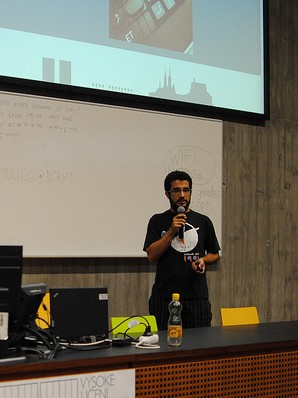
\includegraphics[width=0.275\textwidth]{img/guadec_2013_1.jpg}
    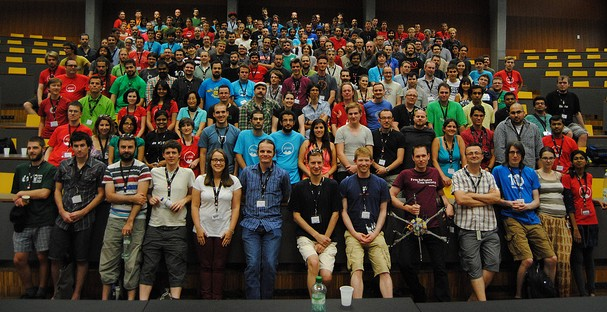
\includegraphics[width=0.715\textwidth]{img/guadec_2013_2.jpg}
    \caption{GUADEC 2013 (Brno)}
    \label{fig:guadec2012}
\end{figure}

Ademais de presentar o proxecto nesta xuntanza participei no evento como voluntario o que me permitiu coñecer a moita xente converténdose nunha experiencia moi enriquecedora tanto profesional como persoalmente.

\subsubsection{Reportes e Feedback}

A Fundación GNOME ponse en contacto comigo a través do email para pedirme que, xa que esta vai ser o aplicativo oficial de GNOME, ten que ter a palabra GNOME no seu nome.

Escribíronse dous reportes un\footnote{\href{http://aquelando.info/guadec-2013/}{GUADEC 2013}} falando da miña experiencia na GUADEC e outro\footnote{\href{http://aquelando.info/searching/}{Searching...}} falando dos avances no programa e pedindo ideas para o novo nome do aplicativo. Daniel Mustieles responde que ``GNOME Translator'' ou ``GNOME Translation Tool'' serían boas opcións.

\subsubsection{Tarefas e seguimento}

A descomposición en tarefas desta iteración é a seguinte:

\begin{enumerate}[label=\bfseries WBS 3.\arabic*]
  \item Deseño e implementación dos iteradores.
  \item Deseño e implementación do sistema de busca.
  \item Interface de usuario.
    \begin{enumerate}[label=\bfseries WBS 2.3.\arabic*]
      \item Resaltado do texto ao facer click nos consellos.
      \item Modificar editor de mensaxes
    \end {enumerate}
  \item Escribir reportes.
\end{enumerate}

Na Figura~\ref{fig:gantt:gsoc1-3} pódese ver o diagrama de Gantt correspondente as tarefas desta iteración.

\begin{figure}[h!]
\centerline{
\begin{ganttchart}[
    %hgrid,
    %inline,
    vgrid={dotted,dashed,dashed,dotted,dotted,dotted,dotted},
    x unit=5mm,
    y unit title=5mm,
    y unit chart=6mm,
    canvas/.style={draw=none},
    time slot format=isodate,
    title/.style={fill=gray, draw=none},
    title label font= \color{white}\scriptsize,
    title left shift=.1,
    title right shift=-.1,
    title top shift=.05,
    title height=.5,
    bar label font=\scriptsize,
    milestone label font=\scriptsize,
    group label font=\scriptsize\bfseries,
    %milestone inline label node/.append style={bottom=5mm},
    %group inline label node/.append style={right=0mm},
    %bar inline label node/.append style={right=0mm}
  ]{2013-07-18}{2013-8-06}
  \gantttitlecalendar{month=name,day} \\
  \ganttbar{Deseño e implementación dos iteradores}{2013-07-18}{2013-07-18} \ganttbar{}{2013-07-21}{2013-07-23} \\
  \ganttbar{Deseño e implementación do sistema de busca}{2013-07-24}{2013-07-25} \ganttbar{}{2013-07-28}{2013-07-29} \\
  \ganttgroup{Interface de usuario}{2013-07-30}{2013-08-4} \\
  \ganttbar{Resaltado do texto ao facer click nos consellos}{2013-07-30}{2013-07-31} \\
  \ganttbar{Modificar editor de mensaxes}{2013-08-1}{2013-08-1}  \ganttbar{}{2013-08-4}{2013-08-4} \\
  \ganttbar{Escribir reportes}{2013-8-5}{2013-8-5} \\
  \ganttlinkedmilestone{Fin terceira iteración}{2013-08-5}{2013-8-5}
\end{ganttchart}}
\caption{Diagrama de Gantt da terceira iteración do GSoC 2013.}
\label{fig:gantt:gsoc1-3}
\end{figure}

Esta iteración planificouse para un total de 65 horas. Nesta ocasión non houbo ningún problema e puideronse executar as tarefas no tempo previsto.

\subsection{Cuarta Iteración: Ficheiros po, Autools, Proxectos, barra de busca}
Esta iteración comeza o 6 de Agosto e remata o 30 do mesmo mes. O obxetivo desta iteración é engadir soporte para ficheiros po, proxectos, autotools e engadir unha barra de busca a interface.

\paragraph{Ficheiros PO}
O obxectivo consiste en implementar o soporte para ficheiros PO pois ata ese momento estábase empregando un mock. Crearanse bindings para a biblioteca gettext-po e implementarase unha subclase da clase abstracta File.

\paragraph{Proxectos}
Durante esta iteración tamén se implementarán os proxectos, definindo proxecto como un conxunto de ficheiros que están na mesma carpeta.

\paragraph{Autotools}
Implementarase tamén o soporte para autotools do proxecto pois ata o momento víñase a empregar un simple ficheiro Makefile.

\paragraph{Interface de usuario}
Crearanse accións para facer e desfacer cambios, navegar a través do documento entre outras cousas. Estas accións poderán ser activadas a través de botóns na interface de usuario ou mediante atallos de teclado que se crearán posteriormente. Ademais engadirase o soporte para abrir ficheiros dende a propia interface e a posibilidade de ver os ficheiros recentes.

\subsubsection{Reportes e feedback}

Falando co anterior \emph{maintainer} de GTranslator a través de IRC, este aporta bastantes consellos sobre o programa como o uso de Autotools ou varios detalles da interface de usuario.

Realizáronse un total de dous reportes\footnote{\href{http://aquelando.info/gsoc-application-status-report/}{GSoC application status report}}\footnote{\href{http://aquelando.info/po-files-projects-navigation-and-other-stuff-i-have-been-doing/}{Po files, projects, navigation and other stuff I have been doing}} pero ninguén escribiu ningún comentario no blogue.

\subsubsection{Tarefas e Seguimento}

As tarefas que se realizaron durante esta iteración foron as seguintes:

\begin{enumerate}[label=\bfseries WBS 4.\arabic*]
  \item Implementación dos ficheiros po.
  \item Implementación de proxectos
  \item Implementación de accións
    \begin{enumerate}[label=\bfseries WBS 4.3.\arabic*]
      \item Accións desfacer-refacer
      \item Accións de navegar polo documento.
    \end{enumerate}
  \item Engadir barra de busca.
  \item Eliminar barra de estado.
  \item Substituir Makefile por Autools.
  \item Internacionalización do programa.
  \item Escribir reportes.
\end {enumerate}

Na Figura~\ref{fig:gantt:gsoc1-4} pódese ver o diagrama de Gantt correspondente a esta iteración.

\begin{figure}[h!]
\centerline{
\begin{ganttchart}[
    %hgrid,
    %inline,
    vgrid={dotted,dotted,dotted,dotted,dotted,dashed,dashed},
    x unit=4.5mm,
    y unit title=5mm,
    y unit chart=6mm,
    canvas/.style={draw=none},
    time slot format=isodate,
    title/.style={fill=gray, draw=none},
    title label font= \color{white}\scriptsize,
    title left shift=.1,
    title right shift=-.1,
    title top shift=.05,
    title height=.5,
    bar label font=\scriptsize,
    milestone label font=\scriptsize,
    group label font=\scriptsize\bfseries,
    %milestone inline label node/.append style={bottom=5mm},
    %group inline label node/.append style={right=0mm},
    %bar inline label node/.append style={right=0mm}
  ]{2013-08-5}{2013-8-30}
  \gantttitlecalendar{month=name,day} \\
  \ganttbar{Implementación dos ficheiros PO}{2013-08-5}{2013-08-9}  \ganttbar{}{2013-08-12}{2013-08-13} \\
  \ganttbar{Implementación de proxectos}{2013-08-14}{2013-08-14} \\
  \ganttgroup{Implementación de accións}{2013-08-15}{2013-08-16} \\
  \ganttbar{Accións desfacer-refacer}{2013-08-15}{2013-08-15} \\
  \ganttbar{Accións de navegar}{2013-08-16}{2013-08-16} \\
  \ganttgroup{Interface de Usuario}{2013-08-19}{2013-08-21} \\
  \ganttbar{Engadir barra de busca}{2013-08-19}{2013-08-20} \\
  \ganttbar{Eliminar barra de estado}{2013-08-21}{2013-08-21} \\
  \ganttbar{Creacion de scripts de Autools}{2013-08-22}{2013-08-23} \ganttbar{}{2013-08-26}{2013-08-28} \\
  \ganttbar{Internacionalización}{2013-08-29}{2013-08-29} \\
  \ganttbar{Escribir reportes}{2013-08-30}{2013-08-30} \\
  \ganttmilestone{Fin cuarta iteración}{2013-08-30}
\end{ganttchart}}
\caption{Diagrama de Gantt da cuarta iteración do GSoC 2013.}
\label{fig:gantt:gsoc1-4}
\end{figure}

Planificáronse un total 100 horas para esta iteración. Tardamos 5 horas máis das previstas en implementar o soporte para Autotools e outras 5 horas adicionais por problemas encontrados na implementación dos bindings da biblioteca de GetText. De igual forma que nos casos anteriores estes problemas resolveronse ampliando a xornada laboral.

\subsection{Quinta Iteración: Preferencias, limpar código e documentación}
Esta iteración comeza o 1 de septembro e remata o 23 do mesmo mes. Durante ela seguirase traballando na interface, limparase o código e crearase algo de documentación de cara a entrega final do Google Summer of Code.

\paragraph{Preferencias}
Empezarase a implementar as preferencias no programa pois ata o momento moitas das opcións estaban \emph{hardcoded}, e dicir escritas directamente no código. Para facer isto farase uso do compoñente de GLib GSettings que permite o almacenamento sinxelo de configuración das aplicacións. Ademais implementarase un dialogo semellante ao empregado en GTranslator para poder modificar estas preferencias.

\paragraph{Mellorar a calidade do código e documentación}
Revisión completa do código para manter un mesmo estilo ao largo de todo o código. Ademais actualizáronse os diagramas UML creados na primeira iteración.

\subsubsection{Reportes e Feedback}
Escribiuse un\footnote{\href{http://aquelando.info/gsoc-final-report/}{GSoC Final Report}} reporte onde se conta o estado da aplicación demostrándoo con un vídeo. O tratarse do último post desa edición do GSoC agradezo a oportunidade que me deu Google para poder estar ese verán traballando en software libre e describo a miña experiencia.

\subsubsection{Tarefas e seguimento}

As tarefas realizadas durante esta iteración foron as seguintes:

\begin{enumerate}[label=\bfseries WBS 5.\arabic*]
  \item Deseño e implementación das preferencias.
  \item Corrixir Clase ficheiro.
  \item Corrixir errores de estilos no código.
  \item Actualizar diagramas UML.
  \item Escribir reportes.
\end {enumerate}

Hai que ter en conta que nesta iteración a cantidade de tempo traballada por día é inferior nalgúns momentos pois en que compatibilizarse co horario lectivo do curso 2013/2014. Na Figura~\ref{fig:gantt:gsoc1-5} pódese ver o diagrama de Gantt que corresponde a esta iteración.

\begin{figure}[h!]
\centerline{
\begin{ganttchart}[
    %hgrid,
    %inline,
    vgrid={dashed,dotted,dotted,dotted,dotted,dotted,dashed},
    x unit=4.5mm,
    y unit title=5mm,
    y unit chart=6mm,
    canvas/.style={draw=none},
    time slot format=isodate,
    title/.style={fill=gray, draw=none},
    title label font= \color{white}\scriptsize,
    title left shift=.1,
    title right shift=-.1,
    title top shift=.05,
    title height=.5,
    bar label font=\scriptsize,
    milestone label font=\scriptsize,
    group label font=\scriptsize\bfseries,
    %milestone inline label node/.append style={bottom=5mm},
    %group inline label node/.append style={right=0mm},
    %bar inline label node/.append style={right=0mm}
  ]{2013-09-1}{2013-9-24}
  \gantttitlecalendar{month=name,day} \\
  \ganttbar{Deseño e implementación das preferencias}{2013-09-2}{2013-09-6} \ganttbar{}{2013-09-9}{2013-09-10} \\
  \ganttbar{Corrixir Clase ficheiro}{2013-09-11}{2013-09-13}  \ganttbar{}{2013-09-16}{2013-09-17} \\
  \ganttbar{Corrixir errores de estilos no código}{2013-09-18}{2013-09-18} \\ 
  \ganttbar{Actualizar diagramas UML}{2013-09-19}{2013-09-20} \\
  \ganttbar{Escribir reportes}{2013-09-23}{2013-09-23} \\
  \ganttmilestone{Fin quinta iteración}{2013-09-23}
\end{ganttchart}}
\caption{Diagrama de Gantt da quinta iteración do GSoC 2013.}
\label{fig:gantt:gsoc1-5}
\end{figure}

Planificaronse un total de 60 horas para resolver as tarefas e non houbo ningún problema en completalas con éxito.

\subsection{Estado ao fin do GSoC 2013}
O finalizar esta iteración o mentor do GSoC avalía correctamente o proxecto presentado polo que o programa é completado con éxito. O programa entregado ten entre outras moitas as seguintes características:

\begin{itemize}
  \item Posibilidade de abrir ficheiros po.
  \item Navegación a través do documento.
  \item Posibilidade de buscar.
  \item Editor con resaltado de sintaxe e de espazos en branco.
  \item Preferencias.
\end{itemize}

Pero tamén presenta algúns fallos:

\begin{itemize}
  \item Lentitude ao cargar ficheiros moi grandes.
  \item Fallo ao gardar un ficheiro.
  \item O aspecto da interface non é satisfactorio.
  \item Problemas ao buscar.
\end{itemize}

Estas limitacións serán eliminadas durante os seguintes períodos.


\section{Primeiro cuatrimestre curso 2013/2014}

Durante este período a implementación do programa faise en paralelo coa vida universitaria. Planifícanse dúas iteracións, a primeira durante o que falta do mes de setembro e o mes de outubro e a segunda durante o final do mes de nobembro. Nestes dous periodos de tempo a carga de traballo das tarefas das materias do curso 2013/2014 é menor e permitenos continuar traballando coa aplicación.

\subsection{Primeira iteración: cambios na interface}
A primeira iteración comprende os últimos días de setembro e o mes de outubro. Durante este tempo farase un redeseño da interface gráfica e implementanse as pistas e os comprobadores:

\paragraph{Interface Gráfica} Pretendese conseguir un mellor resultado do actual. Empregaremos os deseños iniciais que teñen un parecido máis importante a aplicación Virtaal. Reutilizarase os widgets creados combinándoos para conseguir o efecto desexado.


\paragraph{Pistas e Comprobadores} As pistas (\emph{hints}) son posibles traducións para unha cadea determinada. Nesta iteración crearase tanto o panel da interface que permite ver estas pistas como a clase que lle prove as pistas a dita interface. Os comprobadores (\emph{checkers}), por outro lado, apórtanlle pistas de cada tradución feita.

\subsubsection{Presentación GUADEC Hispana 2013 (Madrid)}

A GUADEC Hispana é unha reunión de usuarios e desenvolvedores de GNOME de fala castelá e que serve tamén para a reunión anual (como obriga a lei) da organización GNOME Hispano. Ademais nesta reunión fanse charlas sobre GNOME e outros temas relacionados.

\begin{figure}[h!]
    \centering
    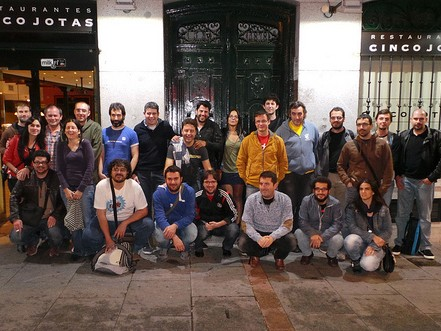
\includegraphics[width=0.495\textwidth]{img/guadec_es_2013_1.jpg}
    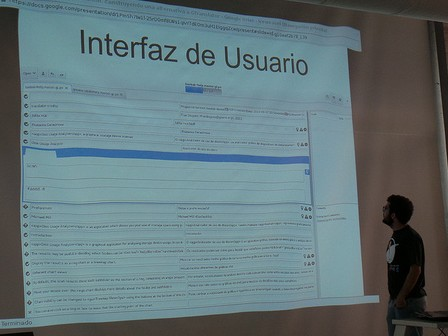
\includegraphics[width=0.495\textwidth]{img/guadec_es_2013_2.jpg}
    \caption{GUADEC Hispana 2013 (Madrid)}
    \label{fig:guadec2012}
\end{figure}

Entre esas charlas tiven a oportunidade de presentar o proxecto polo que os asistentes amosaron o seu interese por que se seguira desenrolando.

\subsubsection{Reportes e feedback}
Escribiuse un reporte\footnote{\href{http://aquelando.info/changing-the-tool-ui/}{Changing the tool UI}} mais ninguén escribiu ningún comentario. Non obstante durante a GUADEC-es houbo xente que se interesou polo programa.

\subsubsection{Tarefas e seguimento}

A descomposición en tarefas para esta iteración é a seguinte:

\begin{enumerate}[label=\bfseries WBS 1.\arabic*]
  \item Implementar Pistas e Provedor de Pistas.
  \item Implementar Comprobador.
  \item Interface de Usuario.
    \begin{enumerate}[label=\bfseries WBS 1.3.\arabic*]
      \item Eliminar biblioteca GDL.
      \item Engadir widget de Pistas.
      \item Misturar lista de mensaxes con editor de mensaxes.
    \end{enumerate}
\end{enumerate}

Hai que ter en conta que ao ter que compatibilizar a realización destas tarefas co horario acadameico o número de horas traballadas cada día é menor que no periodo anterior e non é regular. Na Figura~\ref{fig:gantt:mid1-1} pódese ver o diagrama de Gantt que corresponde a esta iteración.

\begin{figure}[h!]
\centerline{
\begin{ganttchart}[
    vgrid={dotted,dotted,dashed,dashed,dotted,dotted,dotted},
    x unit=4.5mm,
    y unit title=5mm,
    y unit chart=6mm,
    canvas/.style={draw=none},
    time slot format=isodate,
    title/.style={fill=gray, draw=none},
    title label font= \color{white}\scriptsize,
    title left shift=.1,
    title right shift=-.1,
    title top shift=.05,
    title height=.5,
    bar label font=\scriptsize,
    milestone label font=\scriptsize,
    group label font=\scriptsize\bfseries
  ]{2013-09-26}{2013-10-20}
  \gantttitlecalendar{month=name,day} \\
  \ganttbar{Implementar Pistas}{2013-09-26}{2013-09-27} \\
  \ganttbar{Implementar Provedor de Pistas}{2013-09-30}{2013-10-1} \\
  \ganttbar{Implementar Comprobador}{2013-10-2}{2013-10-3} \\
  \ganttgroup{Interface de Usuario}{2013-10-4}{2013-10-17} \\
  \ganttbar{Eliminar biblioteca GDL}{2013-10-4}{2013-10-4}  \ganttbar{}{2013-10-7}{2013-10-8} \\
  \ganttbar{Engadir widget de Pistas}{2013-10-9}{2013-10-11} \\
  \ganttbar{Reimplementar lista de mensaxes}{2013-10-14}{2013-10-17} \\
  \ganttbar{Escribir reportes}{2013-10-18}{2013-10-18} \\
  \ganttmilestone{Fin iteración}{2013-10-18}
\end{ganttchart}}
\caption{Diagrama de Gantt da primeira iteración do primeiro cuatrimestre do curso 2013/2014.}
\label{fig:gantt:mid1-1}
\end{figure}

Para a realización destas tarefas planificáronse 50 horas que se completaron con éxito.

\subsection{Segunda iteración: Refactorizar navegadores e melloras na interface}
Esta iteración sucede no final do mes de novembro. Durante este tempo cambiaraselle o nome ao aplicativo, refactorízase a API para navegar a través do documento e realízaranse pequenos cambios na interface de usuario.

\paragraph{Refactorización dos navegadores} Crearase unha API a nivel de aplicación para movernos a través do documento. O obxectivo é implementar operacións para seleccionar e tamén deseleccionar cadeas e fragmentos destas cadeas a través de todo o documento.

\paragraph{Cambio de nome} Reutilizarase un cambio de nome do aplicativo cambiando o anterior ValaCAT por GNOMECAT. Este cambio é producido polo requirimento por parte da fundación GNOME de que o programa tiña que ter a marca GNOME no seu nome.

\paragraph{Interface de usuario} Farase un redeseño a opción de buscar avanzado para eliminar o dialogo existente e engadir as opción existentes a propia barra de busca.

\subsubsection{Reportes e Feedback}
Escríbese un\footnote{\href{http://aquelando.info/welcome-gnomecat/}{Welcome GnomeCAT}} contando os últimos avances do aplicativo e o cambio de nome. Recibimos un comentario dicindo que GNOME escribese con letras maiúsculas polo que temos que corrixir o programa. Outra xente interesase polo significado de CAT.

\subsubsection{Tarefas e seguimento}

As tarefas realizadas durante esta iteración foron as seguintes:

\begin{enumerate}[label=\bfseries WBS 2.\arabic*]
  \item Cambiar nome do aplicativo.
  \item Refactorizar navegadores.
  \item Interface de usuario.
    \begin{enumerate}[label=\bfseries WBS 2.3.\arabic*]
      \item Redeseño da opción buscar avanzado.
    \end{enumerate}
\end{enumerate}

De igual forma que no caso anterior o feito de estar dentro do periodo lectivo, causa que o número de horas traballadas sexa menor do normal. Na Figura~\ref{fig:gantt:mid1-2} pódese ver o diagrama de Gantt que corresponde a esta iteración.

\begin{figure}[h!]
\centerline{
\begin{ganttchart}[
    vgrid={dotted,dotted,dotted,dotted,dotted,dashed,dashed},
    x unit=4.5mm,
    y unit title=5mm,
    y unit chart=6mm,
    canvas/.style={draw=none},
    time slot format=isodate,
    title/.style={fill=gray, draw=none},
    title label font= \color{white}\scriptsize,
    title left shift=.1,
    title right shift=-.1,
    title top shift=.05,
    title height=.5,
    bar label font=\scriptsize,
    milestone label font=\scriptsize,
    group label font=\scriptsize\bfseries
  ]{2013-11-18}{2013-11-30}
  \gantttitlecalendar{month=name,day} \\
  \ganttbar{Cambiar nome do aplicativo}{2013-11-18}{2013-11-19} \\
  \ganttbar{Refactorizar navegadores}{2013-11-20}{2013-11-22} \\
  \ganttgroup{Interface de usuario}{2013-11-25}{2013-11-28} \\
  \ganttbar{Redeseño da opción buscar avanzado}{2013-11-25}{2013-11-28} \\
  \ganttbar{Escribir reportes}{2013-11-29}{2013-11-29} \\
  \ganttmilestone{Fin segunda iteración}{2013-11-29}
\end{ganttchart}}
\caption{Diagrama de Gantt da segunda iteración do primeiro cuatrimestre do curso 2013/2014.}
\label{fig:gantt:mid1-2}
\end{figure}

Para a realización das tarefas descritas planificanse 35 horas que son suficientes para completalas nos días estipulados.

\subsection{Presentación para o GSoC 2014}
Debido a evidente falta de tempo para completar o programa decídese presentar o programa de novo o proxecto Google Summer of Code. Falase coa coordinadora dos programas de iniciación en GNOME para saber se isto é posible e respóndenos afirmativamente. Como mentor falamos co \emph{maintainer} de GTranslator que nos di que non ten ningún problema en facer de mentor. Presentamos o proxecto e este sae aceptado.

\section{Google Summer of Code 2014}
O Google Summer of Code durante o 2014 dura dende o 19 de maio ata o 11 de agosto un total de 15 semanas. Na planificación realizada cóntanse 13 semanas pois nunha das semanas o curso lectivo 2013/2014 aínda non acabou e na outra realizase o viaxe a GUADEC en Strasbourg. Da mesma forma que no caso anterior planéanse traballar 5 horas diarias o que da un total de 325 horas.

A maior experiencia no programa que estamos a facer permítenos facer unha planificación máis exacta. Faranse un total de cinco iteración de unha duración aproximada de dúas semanas.

\subsection{Primeira iteración: Redeseño UI}

Esta iteración dura dende o 23 de maio ata o 15 xuño. Durante ela fundamentalmente traballaremos nun redeseño da interface.

\paragraph{Interface Gráfica} O obxectivo desta iteración é un novo redeseño da interface. Contactarase cos deseñadores de GNOME a través de IRC para obter algún feedback pola súa parte. Unha vez conseguido, implementarase a nova interface.

\paragraph{Bindings Gettext-PO: Orixes das mensaxes}
A biblioteca gettext-po ten soporte para conseguir os orixes das mensaxes. Nesta iteración tamén se mellorarán os seus bindings para recoller esta característica e tamén a implementaremos na clase PoFile engadindo a propiedade origins que permite obter en que ficheiros e liñas aparece dita cadea.

\subsubsection{Reportes e Feedback}
Escribíronse dous\footnote{\href{http://aquelando.info/gnomecat-progress-report/}{GNOMECAT. Progress report}}\footnote{\href{http://aquelando.info/implementing-the-editing-panel/}{Implementing the Editing Panel}} reportes. En esta iteración hai bastante resposta por parte do usuario. Por unha parte reportase un erro na compilación do programa respondémoslle ao usuario dándolle un \emph{workaround} mentras buscamos o motivo real do problema.

Ademais, o deseñador que fixo os mockups empregados agradece que os esteamos usando e sinala que sería boa idea substituir o menú de selección de idioma actual por algo máis vistoso. Tamén sinala que quedaría ben combinar os botóns de gardar e de volver atrás de forma que un usuario so poida volver a lista de ficheiros abertos cando o ficheiro que está traballando. Anotamos estas dúas ideas en GitHub para implementalas máis tarde.

\subsubsection{Tarefas e seguimento}

As tarefas realizadas durante esta iteración foron:

\begin{enumerate}[label=\bfseries WBS 1.\arabic*]
  \item Creación do ficheiro .desktop.
  \item Mellora de Autotools: xeneración automática das cadeas a traducir.
  \item Interface de Usuario.
    \begin{enumerate}[label=\bfseries WBS 1.3.\arabic*]
      \item Nova estrutura xeral.
      \item Creación da barra de ferramentas.
      \item Panel de edición.
      \item Panel de preferencias.
      \item Panel de perfil.
      \item Panel de benvida.
      \item Menú de aplicativo.
    \end{enumerate}
  \item Bindings Gettext-PO: implementación das orixes dos mensaxes.
  \item Refactorización das buscas.
  \item Refactorización as formas plurais.
\end{enumerate}

Na Figura~\ref{fig:gantt:gsoc2014-1} pódese ver o diagrama de Gantt que corresponde a esta iteración.

\begin{figure}[h!]
\centerline{
\begin{ganttchart}[
    vgrid={dotted,dotted,dashed,dashed,dotted,dotted,dotted},
    x unit=4.5mm,
    y unit title=5mm,
    y unit chart=6mm,
    canvas/.style={draw=none},
    time slot format=isodate,
    title/.style={fill=gray, draw=none},
    title label font= \color{white}\scriptsize,
    title left shift=.1,
    title right shift=-.1,
    title top shift=.05,
    title height=.5,
    bar label font=\scriptsize,
    milestone label font=\scriptsize,
    group label font=\scriptsize\bfseries
  ]{2014-05-22}{2014-6-15}
  \gantttitlecalendar{month=name,day} \\
  \ganttbar{Creación do ficheiro .desktop}{2014-05-23}{2014-05-23} \\
  \ganttgroup{Autotools}{2014-05-26}{2014-05-26} \\
  \ganttbar{Xeneración automática das cadeas a traducir}{2014-05-26}{2014-05-26} \\
  \ganttgroup{Interface de Usuario}{2014-05-27}{2014-06-9} \\
  \ganttbar{Nova estrutura xeral}{2014-05-27}{2014-05-28} \\
  \ganttbar{Creación da barra de ferramentas}{2014-05-29}{2014-05-30} \\
  \ganttbar{Panel de edición}{2014-06-2}{2014-06-3} \\
  \ganttbar{Panel de preferencias}{2014-06-4}{2014-06-4} \\
  \ganttbar{Panel de perfil}{2014-06-5}{2014-06-5} \\
  \ganttbar{Panel de benvida}{2014-06-6}{2014-06-6} \\
  \ganttbar{Menú de aplicativo}{2014-06-9}{2014-06-9} \\
  \ganttgroup{Bindings Gettext-PO}{2014-06-10}{2014-06-10} \\
  \ganttbar{Implementación das orixes dos mensaxes}{2014-06-10}{2014-6-10} \\
  \ganttbar{Refactorización das buscas}{2014-06-11}{2014-06-11} \\
  \ganttbar{Refactorización as formas plurais}{2014-6-12}{2014-6-12} \\
  \ganttbar{Escribir reportes}{2014-06-13}{2014-06-13} \\
  \ganttmilestone{Fin da primeira iteración}{2014-6-13}
\end{ganttchart}}
\caption{Diagrama de Gantt da primeira iteración do GSoC 2014.}
\label{fig:gantt:gsoc2014-1}
\end{figure}

Para facer as tarefas anteriores planifícanse un total de 80 horas. Non son necesarias horas adicionais nesta ocasión.

\subsection{Segunda Iteración: Bindings Gettext-PO e interface}
Esta iteración dura dende o 15 de xuño ata o 6 de xuño. Continuamos mellorando a interface de usuario, implementamos atallos de teclado e engadimos funcionalidade aos bindings de Gettext-PO.

\paragraph{Interface de usuario} Traballarase en implementar atallos de teclado e mellorar o panel de editar perfiles de usuarios dividindo o panel en dous subpaneis. Por último engadirase na interface a opción de obter os orixes de cada mensaxe.

\paragraph{Bindings Gettext-PO} Implementación da opción de modificar as cabeceiras dos ficheiros PO aparte de solucionar algúns erros detectados.

\subsubsection{Reportes e Feedback}

Escríbese un\footnote{\href{http://aquelando.info/keep-working-on-gnomecat/}{Keep working on GNOMECAT}} reporte. So recibimos un comentario sinalando que sería interesante que durante a GUADEC falase con un dos desenvolvedores de GNOME.

\subsubsection{Tarefas e seguimento}

As tarefas realizadas durante esta iteración foron:

\begin{enumerate}[label=\bfseries WBS 2.\arabic*]
  \item Interface de Usuario.
    \begin{enumerate}[label=\bfseries WBS 2.1.\arabic*]
      \item Atallos de teclado.
      \item Widget de Pistas.
      \item Orixes das cadeas.
      \item Mellorar Panel de Perfil.
      \item Mellorar Panel Abrir Ficheiro.
    \end{enumerate}
  \item Arreglar Buscas.
  \item Bindings Gettext-PO.
    \begin{enumerate}[label=\bfseries WBS 2.3.\arabic*]
      \item Xestión de cabeceiras.
      \item Gardado de ficheiros.
    \end{enumerate}
  \item Escribir reportes.
\end{enumerate}

Na Figura~\ref{fig:gantt:gsoc2014-2} pódese ver o diagrama de Gantt que corresponde a esta iteración.

\begin{figure}[h!]
\centerline{
\begin{ganttchart}[
    vgrid={dashed,dotted,dotted,dotted,dotted,dotted,dashed},
    x unit=4.5mm,
    y unit title=5mm,
    y unit chart=6mm,
    canvas/.style={draw=none},
    time slot format=isodate,
    title/.style={fill=gray, draw=none},
    title label font= \color{white}\scriptsize,
    title left shift=.1,
    title right shift=-.1,
    title top shift=.05,
    title height=.5,
    bar label font=\scriptsize,
    milestone label font=\scriptsize,
    group label font=\scriptsize\bfseries
  ]{2014-06-15}{2014-7-6}
  \gantttitlecalendar{month=name,day} \\
  \ganttgroup{Interface de Usuario}{2014-06-16}{2014-06-26} \\
  \ganttbar{Atallos de teclado}{2014-06-16}{2014-06-17} \\
  \ganttbar{Widget de Pistas}{2014-06-18}{2014-06-19} \\
  \ganttbar{Orixes das cadeas}{2014-06-20}{2014-06-20} \\
  \ganttbar{Mellorar Panel Perfil}{2014-6-23}{2014-6-24} \\
  \ganttbar{Mellorar Panel Abrir Ficheiro}{2014-6-25}{2014-6-26} \\
  \ganttbar{Arreglar buscas}{2014-06-27}{2014-06-27} \\
  \ganttgroup{Bindings Gettext-PO}{2014-06-30}{2014-07-3} \\
  \ganttbar{Xestión de cabeceiras}{2014-06-30}{2014-07-1} \\
  \ganttbar{Gardado de ficheiros}{2014-07-2}{2014-07-3} \\
  \ganttbar{Escribir reportes}{2014-7-4}{2014-7-4} \\
  \ganttmilestone{Fin Segunda iteración}{2014-7-4}
\end{ganttchart}}
\caption{Diagrama de Gantt da segunda iteración do GSoC 2014.}
\label{fig:gantt:gsoc2014-2}
\end{figure}

Planificamos un total de 75 horas para esta iteración. Necesitamos 3 horas adicionais para resolver algúns problemas encontrados coa implementación dos bindings para a biblioteca Gettext-PO.

\subsection{Terceira Iteración: Perfiles de usuario e interface}
Esta iteración dura dende o 7 de Xullo ao 16 do mesmo mes. Melloramos algo a interface de usuario e implementamos algún detalle que faltaba no sistema de perfiles.

\paragraph{Interface de usuario: Barra de notificación} Implementarase un sistema de notificacións para alertar ao usuario de certos eventos no programa como por exemplo cando os parámetros de busca non xeran ningún resultado. Para iso empregaremos o widget de GTK GtkInfoBar que amosaremos durante 3 segundos.

\paragraph{Perfiles de usuario} Implementarase a funcionalidade de activar perfiles e engadirase un botón a interface para permitir borrar e activar perfiles.

\subsubsection{Reportes e Feedback}

Escribese un\footnote{\href{http://aquelando.info/details-and-more-details/}{Details and more details}} reporte pero non recibimos feedback por parte dos tradutores nesta iteración.

\subsubsection{Tarefas e seguimento}

As tarefas realizadas durante esta iteración foron:

\begin{enumerate}[label=\bfseries WBS 3.\arabic*]
  \item Interface de usuario: barra de notificación.
  \item Perfiles de usuario.
    \begin{enumerate}[label=\bfseries WBS 3.2\arabic*]
      \item Función borrar perfil.
      \item Función activar perfil.
    \end{enumerate}
  \item Modificar ficheiro das formas plurais.
\end{enumerate}

Na Figura~\ref{fig:gantt:gsoc2014-3} pódese ver o diagrama de Gantt que corresponde a esta iteración.

\begin{figure}[h!]
\begin{ganttchart}[
    vgrid={dashed,dashed,dotted,dotted,dotted,dotted,dotted},
    x unit=4.5mm,
    y unit title=5mm,
    y unit chart=6mm,
    canvas/.style={draw=none},
    time slot format=isodate,
    title/.style={fill=gray, draw=none},
    title label font= \color{white}\scriptsize,
    title left shift=.1,
    title right shift=-.1,
    title top shift=.05,
    title height=.5,
    bar label font=\scriptsize,
    milestone label font=\scriptsize,
    group label font=\scriptsize\bfseries
  ]{2014-07-5}{2014-7-17}
  \gantttitlecalendar{month=name,day} \\
  \ganttgroup{Interface de usuario}{2014-07-7}{2014-07-7} \\
  \ganttbar{Barra de notificación}{2014-07-7}{2014-07-7} \\
  \ganttgroup{Perfiles de usuario}{2014-07-8}{2014-07-10} \\
  \ganttbar{Función borrar perfil}{2014-07-8}{2014-07-8} \\
  \ganttbar{Función activar perfil}{2014-07-9}{2014-07-10} \\
  \ganttgroup{Refactorizar API Formas Plurais}{2014-07-11}{2014-7-11} \\
  \ganttbar{Modificar ficheiro das formas plurais}{2014-7-11}{2014-7-11} \\
  \ganttbar{Mellorar Busca}{2014-07-14}{2014-07-15} \\
  \ganttbar{Escribir reportes}{2014-07-16}{2014-07-16} \\
  \ganttmilestone{Fin terceira iteración}{2014-7-16}
\end{ganttchart}
\caption{Diagrama de Gantt da terceira iteración do GSoC 2014.}
\label{fig:gantt:gsoc2014-3}
\end{figure}

Para completar as tarefas anteriores planificamos 40 horas que foron suficientes para conseguir rematar as tarefas con éxito.

\subsection{Cuarta Iteración: Plugins e GUADEC}
Esta iteración dura dende o 16 de Xullo ata o 5 de Agosto tendo a GUADEC polo medio. Conseguimos implementar o motor de plugins e creamos algúns plugins de exemplo.

\paragraph{Plugins} Engadiremos o soporte de plugins o programa. Por unha parte incorporaremos un motor de plugins e refactorizaremos o código para que certas partes do mesmo deixen de depender da interface de usuario. Ademais modificaremos a configuración de Autotools para que compile os plugins.

\subsubsection{Presentación GUADEC 2014 (Strasbourg)}
Da mesma forma que na edición anterior acudimos a GUADEC, a reunión de programadores e usuarios de GNOME en Europa. Desta vez celébrase en Strasbourg.

\begin{figure}[h!]
    \centering
    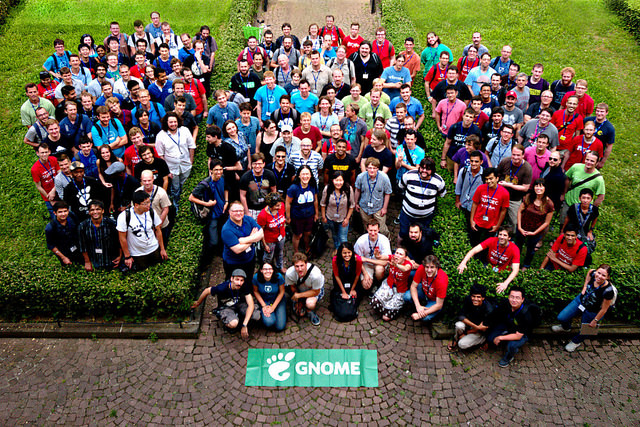
\includegraphics[width=0.999\textwidth]{img/guadec_2014.jpg}
    \caption{GUADEC 2014 (Strasbourg)}
    \label{fig:guadec2012}
\end{figure}

Tamén temos a oportunidade de presentar o proxecto ante a comunidade GNOME nunha charla lóstrego de 3 minutos onde explicaremos os novos cambios na interface, a implementación e plugins e as novas características implementadas.

\subsubsection{Reportes e Feedback}

Escribese un\footnote{\href{http://aquelando.info/api-guadec-and-big-files/}{API, GUADEC and big files}} reporte. Ninguén fai un comentario no blogue sobre o programa pero durante a GUADEC fálase con algún desenvolvedor que nos da consellos sobre algún dos problemas que temos. Marina Zhurakhinskaya recoméndanos falar con Allan Day que é o deseñador líder de GNOME para que nos diga se hai algo que debemos mellorar no deseño do aplicativo.

\subsubsection{Tarefas e seguimento}

As tarefas realizadas duarnte esta iteración foron:

\begin{enumerate}[label=\bfseries WBS 4.\arabic*]
  \item Melloras en Autools
  \item Interface de usuario: \emph{scrolling} nas buscas.
  \item Implementación de plugins.
  \item Refactorizar clase File: evitar dependencias coa interface.
\end{enumerate}

Na Figura~\ref{fig:gantt:gsoc2014-4} pódese ver o diagrama de Gantt que corresponde a esta iteración.

\begin{figure}[h!]
\centerline{
\begin{ganttchart}[
    vgrid={dotted,dotted,dotted,dashed,dashed,dotted,dotted},
    x unit=4.5mm,
    y unit title=5mm,
    y unit chart=6mm,
    canvas/.style={draw=none},
    time slot format=isodate,
    title/.style={fill=gray, draw=none},
    title label font= \color{white}\scriptsize,
    title left shift=.1,
    title right shift=-.1,
    title top shift=.05,
    title height=.5,
    bar label font=\scriptsize,
    milestone label font=\scriptsize,
    group label font=\scriptsize\bfseries
  ]{2013-7-16}{2013-8-6}
  \gantttitlecalendar{month=name,day} \\
  \ganttgroup{Implementación de plugins}{2013-07-16}{2013-07-25} \\
  \ganttbar{Implementación de motor de plugins}{2013-07-16}{2013-07-17} \\
  \ganttgroup{Biblioteca GNOMECAT}{2013-07-18}{2013-07-22} \\
  \ganttbar{Refactorizar clase File}{2013-07-18}{2013-07-18}  \ganttbar{}{2013-07-21}{2013-07-21} \\
  \ganttbar{Refactorizar clase Language}{2013-07-22}{2013-07-22} \\
  \ganttbar{Modificar Autotools para compilar plugins}{2013-07-23}{2013-07-23} \\
  \ganttbar{Plugin de exemplo de comprobador}{2013-07-24}{2013-07-24} \\
  \ganttbar{Plugin de exemplo de proveedor de suxerencias}{2013-07-25}{2013-07-25} \\
  \ganttbar{Refactorizar Navegadores}{2013-07-28}{2013-07-29} \\
  \ganttbar{Interface de usuario: scrolling nas buscas}{2013-07-30}{2013-07-31} \\
  \ganttbar{Mellorar o rendemento con ficheiros grandes}{2013-08-1}{2013-08-1}  \ganttbar{}{2013-08-4}{2013-08-4} \\
  \ganttbar{Escribir reportes}{2013-08-5}{2013-08-5} \\
  \ganttmilestone{Fin cuarta iteración}{2013-8-5}
\end{ganttchart}}
\caption{Diagrama de Gantt da cuarta iteración do GSoC 2014.}
\label{fig:gantt:gsoc2014-4}
\end{figure}

Planificamos 75 horas para as tarefas desta iteración. Precisamos 5 horas adicionais para modificar os scripts de Autotools que permiten a compilación dos plugins. Para non incrementar o número de días desta iteración aumentamos o número de horas que traballamos determinados días.


\subsection{Quinta Iteración: Detalles finais e escribir documentación}
Esta iteración dura dende o 5 de Agosto ata o 15 do mesmo mes. Nela puliremos algún detalle da interface e melloraremos a calidade do código e a documentación.

\paragraph{Documentación e limpar código} O obxectivo é facer unha revisión do código para que este manteña un mesmo estilo. Ademais actualizarase a documentación existente e crearase algunha nova.

\paragraph{Interface: Lista de mensaxes} Intentarase mellorar o rendemento da lista de mensaxes que detectamos que non funciona correctamente con ficheiros grandes. Este é un problema que temos dende a primeira edición do GSoC. Ademais engadiremos a función de filtrar e ordenar mensaxes.

\subsubsection{Reportes e Feedback}
Nesta ocasión non se escriben reportes mais si que recibimos feedback de algún tradutor a través do correo electrónico. As cousas que estes tradutores consideran que se deben mellorar son as seguintes:

\begin{itemize}
   \item Mellora dos atallos de teclado.
\end{itemize}

Ademais falamos con Allan Day que nos di que cando poida fará unha revisión da interface de usuario do programa.

\subsubsection{Tarefas e seguimento}

As tarefas realizadas durante esta iteración foron:

\begin{enumerate}[label=\bfseries WBS 5.\arabic*]
  \item Documentación.
  \item Limpar código.
  \item Interface de usuario: Refactorizar lista de mensaxes.
    \begin{enumerate}[label=\bfseries WBS 5.3.\arabic*]
      \item Implementar novo widget de lista de mensaxes.
      \item Implementar filtros para lista de mensaxes.
      \item Implementar a función de ordenar para mensaxes.
    \end{enumerate}
  \item Melloras en Autotools.
\end{enumerate}

Na Figura~\ref{fig:gantt:gsoc2014-5} pódese ver o diagrama de Gantt que corresponde a esta iteración.

\begin{figure}[h!]
\centerline{
\begin{ganttchart}[
    vgrid={dotted,dotted,dotted,dotted,dashed,dashed,dotted},
    x unit=4.5mm,
    y unit title=5mm,
    y unit chart=6mm,
    canvas/.style={draw=none},
    time slot format=isodate,
    title/.style={fill=gray, draw=none},
    title label font= \color{white}\scriptsize,
    title left shift=.1,
    title right shift=-.1,
    title top shift=.05,
    title height=.5,
    bar label font=\scriptsize,
    milestone label font=\scriptsize,
    group label font=\scriptsize\bfseries
  ]{2013-08-4}{2013-8-16}
  \gantttitlecalendar{month=name,day} \\
  \ganttgroup{Interface de usuario: Refactorizar lista de mensaxes}{2013-08-5}{2013-08-11} \\
  \ganttbar{Implementar novo widget de lista de mensaxes}{2013-08-5}{2013-08-7} \\
  \ganttbar{Implementar filtros para lista de mensaxes}{2013-08-10}{2013-08-10} \\
  \ganttbar{Implementar a función de ordenar para mensaxes}{2013-08-11}{2013-08-11} \\
  \ganttbar{Melloras en Autotools}{2013-08-12}{2013-08-12} \\
  \ganttbar{Documentación}{2013-08-13}{2013-08-13} \\
  \ganttbar{Limpar código}{2013-08-14}{2013-08-14} \\
  \ganttmilestone{Fin quinta iteración}{2013-8-14}
\end{ganttchart}}
\caption{Diagrama de Gantt da quinta iteración do GSoC 2014.}
\label{fig:gantt:gsoc2014-5}
\end{figure}

Para resolver as tarefas desta iteración necesitaremos 40 horas. Non se necesitan horas adicionais para completar o traballo.
